\documentclass[11pt,a4paper]{article}
\usepackage[margin=2.2cm]{geometry}
\usepackage{fontspec,booktabs,graphicx,amsmath}
\setmainfont{DejaVu Serif}
\begin{document}
\begin{center}\Large Examen 1 — Minería de Textos\\[8pt]
Luis Alfredo Ramírez Maza\\ Universidad Nacional Autónoma de México\\
Facultad de Estudios Superiores Acatlán\\
Licenciatura en Ciencia de Datos\\ 11 de noviembre de 2026\end{center}
\section*{1. Portada compacta}
Esqueleto técnico del primer corte. Prosa pendiente de aprobación humana.
\section*{2. Datos, limpieza y segmentación}
Esqueleto técnico del primer corte. Prosa pendiente de aprobación humana.
\par\medskip\noindent\begin{tabular}{ll}
\toprule
Indicador & Valor \\ \midrule
Pasajes & 127739 \\
Discursos excluidos & 5 \\
Ventanas cortas descartadas & 63384 \\
\bottomrule\end{tabular}\par\medskip

\newpage
\section*{3. Preprocesamiento e índice invertido}
Esqueleto técnico del primer corte. Prosa pendiente de aprobación humana.
\section*{4. Ranking y evaluación de IR}
Esqueleto técnico del primer corte. Prosa pendiente de aprobación humana.
\par\medskip\noindent\begin{tabular}{llll}
\toprule
modelo & P@5 & P@10 & MAP \\ \midrule
bm25\_con\_filtro & 0.7600 & 0.7700 & 0.6150 \\
bm25\_sin\_filtro & 0.7600 & 0.7500 & 0.5922 \\
tfidf\_con\_filtro & 0.6600 & 0.5800 & 0.3998 \\
tfidf\_sin\_filtro & 0.6800 & 0.6000 & 0.4131 \\
\bottomrule\end{tabular}\par\medskip

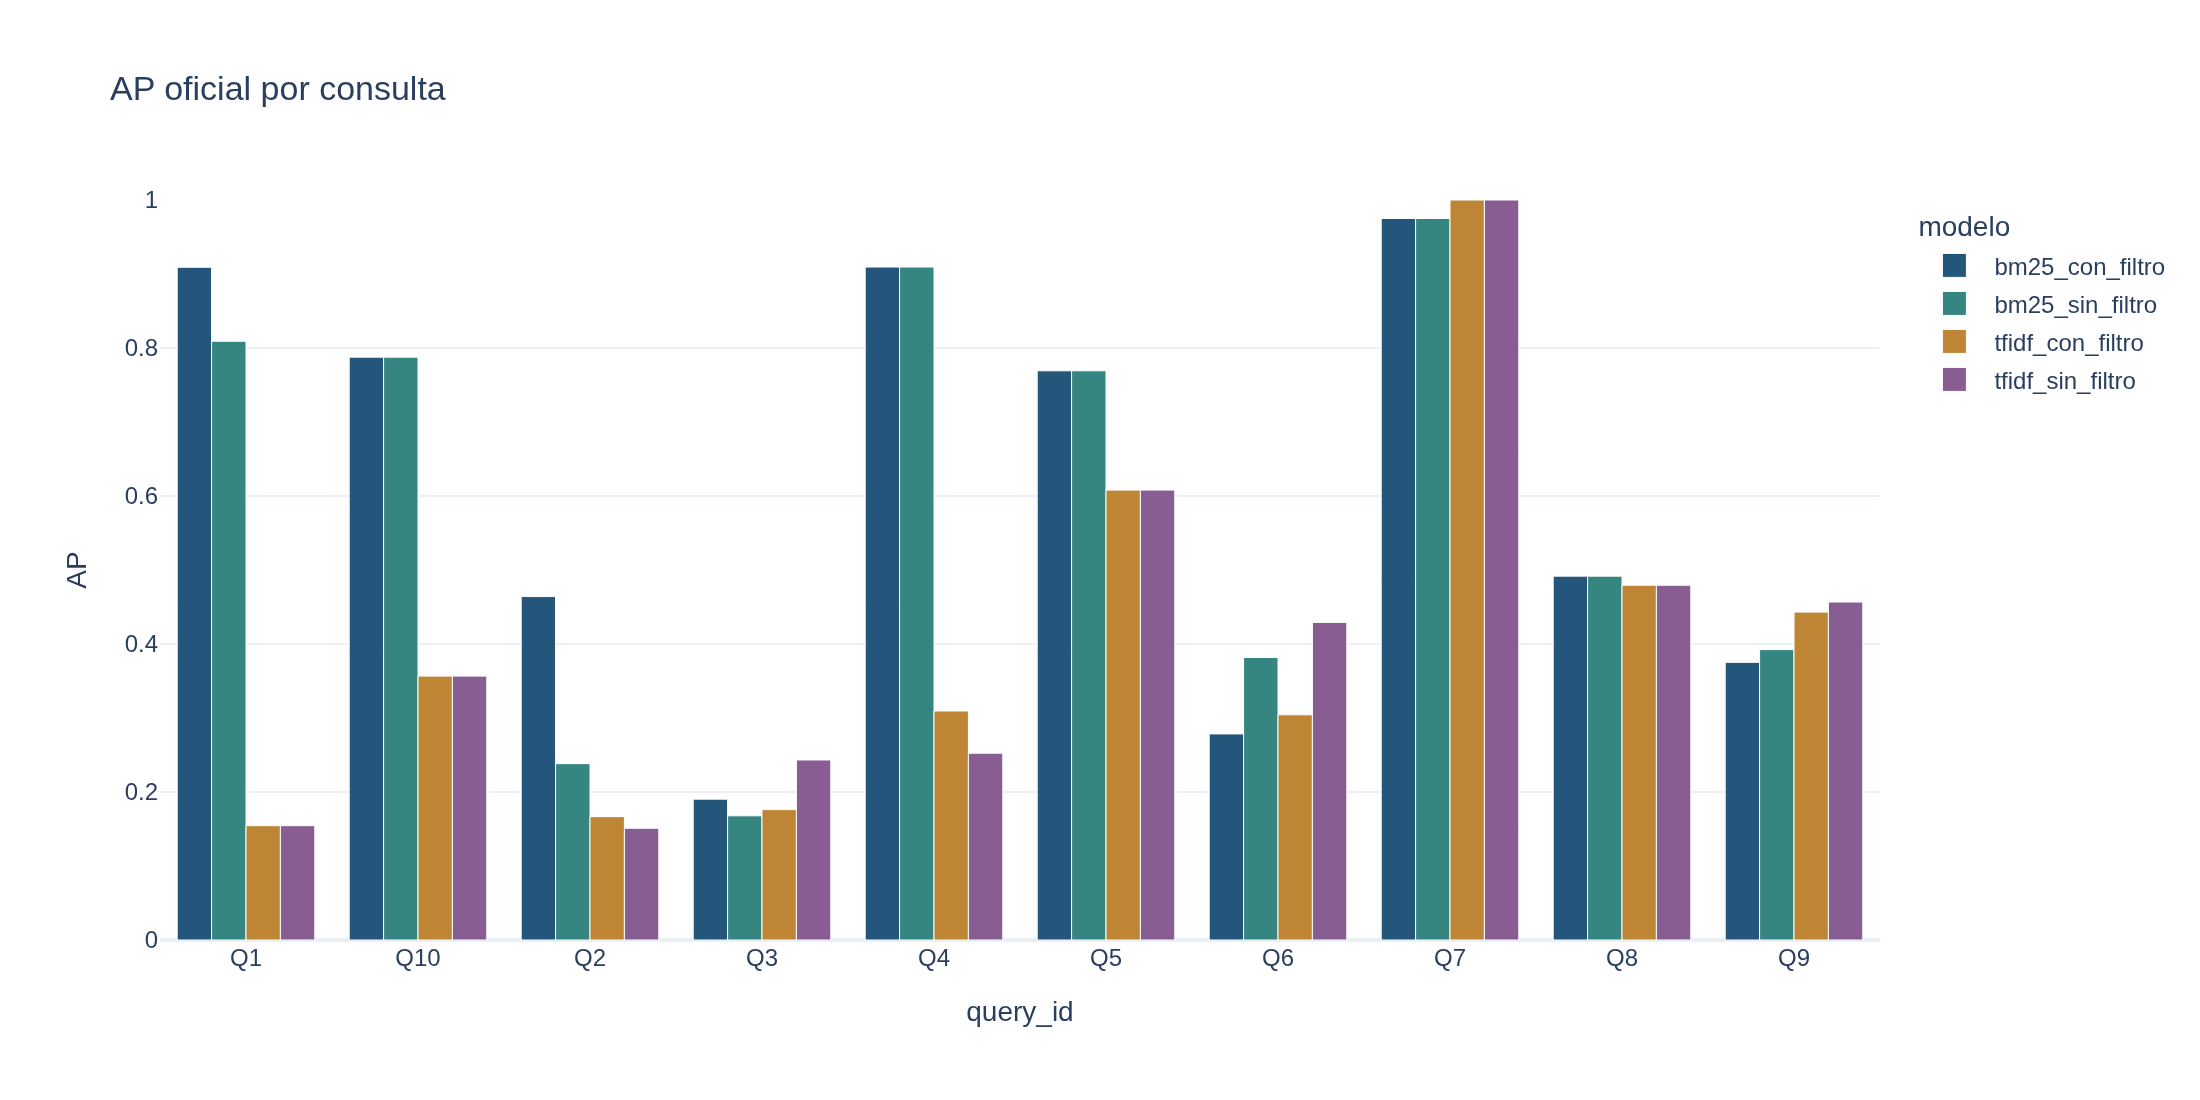
\includegraphics[width=0.9\linewidth,height=6cm,keepaspectratio]{figuras/ir_ap_por_consulta.png}
\newpage
\section*{5. Extracción con reglas y con modelo}
Esqueleto técnico del primer corte. Prosa pendiente de aprobación humana.
\section*{6. Evaluación de IE y análisis de errores}
Esqueleto técnico del primer corte. Prosa pendiente de aprobación humana.
\par\medskip\noindent\begin{tabular}{llll}
\toprule
metodo & precision & recall & f1 \\ \midrule
regla & 0.7245 & 0.5145 & 0.6017 \\
modelo & 0.6947 & 0.6594 & 0.6766 \\
combinado & 0.6257 & 0.8116 & 0.7066 \\
\bottomrule\end{tabular}\par\medskip

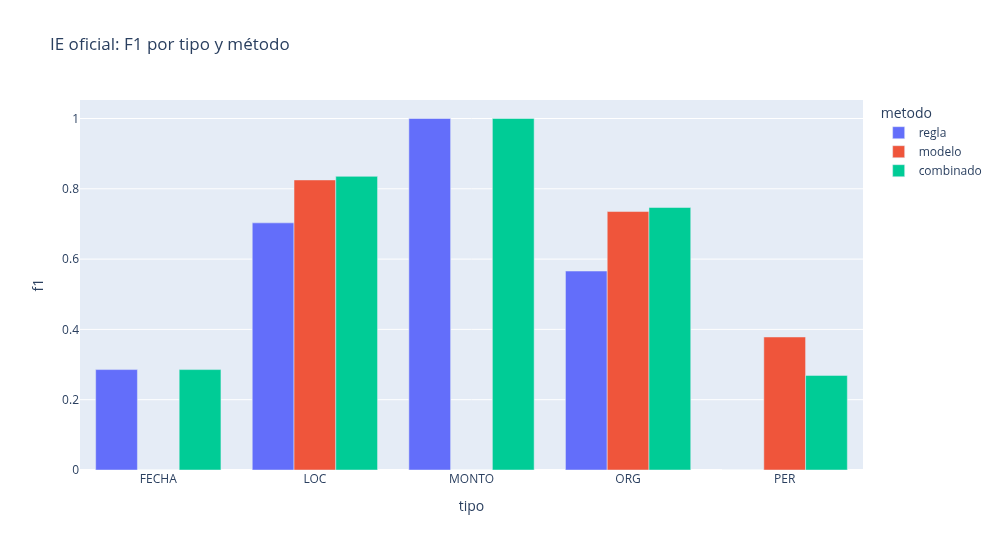
\includegraphics[width=0.85\linewidth,height=5cm,keepaspectratio]{figuras/ie_f1_por_tipo_metodo.png}
\newpage
\section*{7. Tablas de respuesta}
Esqueleto técnico del primer corte. Prosa pendiente de aprobación humana.
\small\par\medskip\noindent\begin{tabular}{llll}
\toprule
query\_id & Ambiguas & Sin evidencia & Respaldadas \\ \midrule
Q1 & 11 & 1 & 4 \\
Q10 & 93 & 0 & 28 \\
Q2 & 17 & 0 & 15 \\
Q3 & 23 & 0 & 1 \\
Q4 & 46 & 0 & 25 \\
Q5 & 32 & 0 & 4 \\
Q6 & 20 & 0 & 7 \\
Q7 & 35 & 1 & 1 \\
Q8 & 10 & 1 & 6 \\
Q9 & 35 & 0 & 35 \\
\bottomrule\end{tabular}\par\medskip
\normalsize
\section*{8. Uso de IA, limitaciones y reproducibilidad}
Esqueleto técnico del primer corte. Prosa pendiente de aprobación humana.
\end{document}